\documentclass{beamer}
\usetheme{Madrid}
\usecolortheme{whale}
\usepackage{graphicx}
\usepackage{listings}
\usepackage{xcolor}
\usepackage{ragged2e}
\usepackage{tikz}

\lstset{
  basicstyle=\small\ttfamily,
  breaklines=true,
  frame=single,
  showstringspaces=false,
  keywordstyle=\color{blue},
  commentstyle=\color{green!60!black},
  stringstyle=\color{red},
}

\title{Automation and Orchestration in Secure Operations}
\subtitle{Enhancing Security Through Programmatic Controls}
\author{Security Operations Course}
\date{\today}

\begin{document}

\begin{frame}
  \titlepage
\end{frame}

% Slide 1
\begin{frame}
  \frametitle{Understanding Automation and Orchestration in Security Operations}
  
  \begin{itemize}
    \item \textbf{Automation} refers to technology that performs tasks with minimal human intervention to increase efficiency and reduce errors.
    \item \textbf{Orchestration} coordinates multiple automated tasks across different systems to create complex workflows.
    \item Security automation helps organizations respond faster to threats while maintaining consistency in security controls.
    \item Today's security challenges require speed and scale that human-only approaches cannot achieve.
  \end{itemize}
  
  \begin{alertblock}{Key Distinction}
    Automation focuses on individual tasks, while orchestration connects these tasks into comprehensive security processes.
  \end{alertblock}
\end{frame}

% Slide 2
\begin{frame}
  \frametitle{The Security Landscape: Why Automation Matters Now}
  
  \begin{itemize}
    \item Modern organizations face an expanding attack surface with cloud services, remote work, and numerous endpoints.
    \item The volume of security alerts has grown exponentially, creating alert fatigue for security teams.
    \item \textbf{Mean time to detect (MTTD)} and \textbf{mean time to respond (MTTR)} are critical metrics that automation can significantly improve.
    \item Skilled security professionals are in short supply, making efficiency through automation essential.
  \end{itemize}
  
  \begin{exampleblock}{Example: Alert Volume}
    A typical enterprise security operations center (SOC) might process over 10,000 alerts per day, making manual triage impossible.
  \end{exampleblock}
\end{frame}

% Slide 3
\begin{frame}
  \frametitle{From Manual to Automated: The Evolution of Security Operations}
  
  \begin{itemize}
    \item Security operations have evolved from reactive manual processes to proactive automated systems.
    \item Early security focused on perimeter defense, while modern approaches require continuous monitoring and rapid response.
    \item \textbf{Security orchestration, automation, and response (SOAR)} platforms represent the current evolution of security automation.
    \item Organizations typically progress through maturity levels, from basic scripting to full orchestration.
  \end{itemize}
  
  \begin{table}
    \begin{tabular}{|l|l|}
      \hline
      \textbf{Security Evolution Stage} & \textbf{Primary Approach} \\
      \hline
      Traditional & Manual review and response \\
      Early Automation & Basic scripting and scheduled tasks \\
      Current Practice & Integrated SOAR platforms \\
      Future Direction & AI-driven autonomous security \\
      \hline
    \end{tabular}
  \end{table}
\end{frame}

% Slide 4
\begin{frame}
  \frametitle{Key Objectives: What We'll Cover Today}
  
  \begin{itemize}
    \item Understand the fundamental importance of automation in modern security operations.
    \item Explore practical use cases for security automation across different operational areas.
    \item Examine the tangible benefits that automation brings to security teams and organizations.
    \item Consider important challenges and limitations when implementing security automation.
  \end{itemize}
  
  \begin{columns}[t]
    \column{0.5\textwidth}
    \textbf{Topics We'll Explore:}
    \begin{itemize}
      \item User \& Resource Provisioning
      \item Guard Rails \& Security Groups
      \item Incident Response Automation
      \item Access Management
      \item CI/CD Security Integration
    \end{itemize}
    
    \column{0.5\textwidth}
    \textbf{Benefits We'll Discuss:}
    \begin{itemize}
      \item Efficiency Gains
      \item Consistent Security Baselines
      \item Secure Scaling
      \item Employee Retention
      \item Response Time Improvements
    \end{itemize}
  \end{columns}
\end{frame}

% Slide 5
\begin{frame}
  \frametitle{Security at Scale: The Automation Imperative}
  
  \begin{itemize}
    \item Modern enterprises manage thousands of users, devices, and applications that require consistent security controls.
    \item Manual security operations simply cannot scale to address the volume and velocity of modern threats.
    \item \textbf{Attack scaling} occurs when threat actors use automation to launch attacks, requiring automated defenses.
    \item Cloud environments with dynamic resources demand automated security that can adapt in real-time.
  \end{itemize}
  
  \begin{block}{Scale By The Numbers}
    \begin{itemize}
      \item Average enterprise: 1,000+ applications
      \item Typical cloud environment: 10,000+ resources
      \item Daily login events: 50,000+ authentications
      \item Security logs generated daily: 10+ GB
    \end{itemize}
  \end{block}
\end{frame}

% Slide 6
\begin{frame}
  \frametitle{Human Error vs. Automated Consistency}
  
  \begin{itemize}
    \item Human operators, regardless of training, make errors when performing repetitive security tasks.
    \item Studies show that approximately 95\% of cybersecurity breaches involve human error as a contributing factor.
    \item \textbf{Configuration drift} occurs when manual changes accumulate, creating security inconsistencies over time.
    \item Automated processes perform identical operations consistently, eliminating variation and reducing errors.
  \end{itemize}
  
\end{frame}

% Slide 7
\begin{frame}[fragile]
  \frametitle{Reaction Time: Minutes vs. Milliseconds}
  
  \begin{itemize}
    \item \textbf{Dwell time} is the period between a breach and its detection, averaging 277 days in 2020 according to IBM.
    \item Modern attacks like ransomware can encrypt an entire network in under 45 minutes once they begin execution.
    \item Human analysts typically take 30+ minutes to investigate even a straightforward security alert.
    \item Automated security responses can execute countermeasures in milliseconds, containing threats before they spread.
  \end{itemize}
  
  \begin{block}{Simple Python automation example}
    \scriptsize
    \begin{semiverbatim}
# Example of automated threat response
def detect_and_respond(alert):
    if alert.severity >= CRITICAL:
        # Immediate automated response
        quarantine_device(alert.source_ip)
        block_traffic(alert.destination_ip)
        notify_security_team(alert)
        # Total execution time: ~200ms
    \end{semiverbatim}
  \end{block}
\end{frame}

% Slide 8
\begin{frame}
  \frametitle{Establishing a Security Foundation Through Automation}
  
  \begin{itemize}
    \item \textbf{Security posture} refers to an organization's overall cybersecurity strength, which automation helps maintain consistently.
    \item Automation creates a reliable security foundation by ensuring that baseline controls are always enforced.
    \item Automated systems continuously validate and correct security configurations, preventing security degradation.
    \item Documentation of security processes happens automatically when using orchestration platforms, improving compliance.
  \end{itemize}
  
  \begin{alertblock}{Foundation Elements That Should Be Automated}
    \scriptsize
    \begin{enumerate}
      \item Identity and access management processes
      \item Vulnerability scanning and patch management
      \item Configuration management and compliance checking
      \item Basic security monitoring and alerting
    \end{enumerate}
  \end{alertblock}
\end{frame}

% Slide 9
\begin{frame}
  \frametitle{User Provisioning: Automating Account Creation and Access}
  
  \begin{itemize}
    \item User provisioning involves creating, modifying, disabling, and deleting user accounts across systems.
    \item \textbf{Identity lifecycle management} ensures users have appropriate access throughout their employment journey.
    \item Manual provisioning leads to inconsistent permissions, orphaned accounts, and compliance violations.
    \item Automated provisioning ensures consistent application of access policies and immediate revocation upon termination.
  \end{itemize}
  
  \begin{exampleblock}{Example: Onboarding Automation}
    \scriptsize
    When HR adds a new employee, an automated workflow:
    \begin{enumerate}
      \item Creates accounts in all relevant systems
      \item Assigns role-based permissions
      \item Provisions necessary resources
      \item Schedules required security training
    \end{enumerate}
  \end{exampleblock}
\end{frame}

% Slide 10
\begin{frame}[fragile]
  \frametitle{Resource Provisioning: Infrastructure as Code}
  
  \begin{itemize}
    \item \textbf{Infrastructure as Code (IaC)} defines infrastructure resources using configuration files rather than manual setup.
    \item Traditional resource provisioning involved manual configuration that was error-prone and difficult to reproduce.
    \item IaC ensures that every server, network, and service is deployed with security controls pre-configured.
    \item Version control for infrastructure code provides audit trails and enables security reviews before deployment.
  \end{itemize}
  
  \begin{block}{Terraform example for secure VM provisioning}
    \tiny
    \begin{semiverbatim}
resource "aws_instance" "web_server" \{
  ami           = "ami-12345678"
  instance_type = "t2.micro"
  
  # Security configuration
  vpc_security_group_ids = [aws_security_group.web_sg.id]
  
  # Encrypt root volume
  root_block_device \{
    encrypted = true
  \}
  
  # Enable detailed monitoring
  monitoring = true
\}
    \end{semiverbatim}
  \end{block}
\end{frame}

% Slide 11
\begin{frame}
  \frametitle{Guard Rails: Automated Boundaries for Security}
  
  \begin{itemize}
    \item \textbf{Guard rails} are automated controls that prevent insecure actions while allowing legitimate operations to proceed.
    \item Unlike blockers that stop all activity, guard rails provide safety without impeding productivity.
    \item Examples include preventing deployment of unencrypted databases or blocking public access to sensitive storage.
    \item Effective guard rails provide immediate feedback to users about why an action was prevented.
  \end{itemize}
  
  \begin{table}
    \scriptsize
    \begin{tabular}{|p{0.45\textwidth}|p{0.45\textwidth}|}
      \hline
      \textbf{Without Guard Rails} & \textbf{With Guard Rails} \\
      \hline
      Users can create cloud storage with public access & System automatically enforces private-only access \\
      \hline
      Developers can deploy applications without security scanning & Pre-deployment hooks require security validation \\
      \hline
      Administrators can modify firewall rules without review & Changes require approval or follow predefined patterns \\
      \hline
      Resources can be created without proper tagging & System enforces mandatory security classification tags \\
      \hline
    \end{tabular}
  \end{table}
\end{frame}

% Slide 12
\begin{frame}
  \frametitle{Security Groups: Dynamically Managing Access Control}
  
  \begin{itemize}
    \item \textbf{Security groups} are logical collections of users or resources that share common access requirements.
    \item Dynamic security groups automatically update memberships based on user attributes or resource properties.
    \item Automation ensures that access control remains accurate as users change roles or resources are modified.
    \item Centralized security group management reduces administrative overhead and improves security consistency.
  \end{itemize}
  
  \begin{block}{Dynamic Security Group Logic}
    \scriptsize
    \begin{align}
      \text{Finance\_Access} &= \{x \mid x \in \text{Employees} \wedge \text{Department}(x) = \text{Finance}\} \\
      \text{Admin\_Access} &= \{x \mid x \in \text{Employees} \wedge \text{Role}(x) = \text{Administrator}\} \\
      \text{PCI\_Systems} &= \{s \mid s \in \text{Systems} \wedge \text{DataClass}(s) = \text{PCI}\}
    \end{align}
  \end{block}
\end{frame}

% Slide 13
\begin{frame}
  \frametitle{Ticket Creation: Streamlining Incident Response}
  
  \begin{itemize}
    \item \textbf{Security incident tickets} provide structured documentation and workflow management for security events.
    \item Automated ticket creation ensures that all security alerts are properly tracked without analyst intervention.
    \item Enrichment automation adds context to tickets by gathering related information about affected assets.
    \item Proper ticket categorization through automation helps prioritize response efforts and allocate resources effectively.
  \end{itemize}
  
  \begin{exampleblock}{Enriched Ticket Example}
    \tiny
    \textbf{Automated Ticket}: Multiple failed login attempts \\
    \textbf{Severity}: Medium (Auto-calculated) \\
    \textbf{Asset}: finance-server-01 \\
    \textbf{Auto-enriched context}:
    \begin{itemize}
      \item Critical system handling financial data
      \item Source IP: 185.22.xx.xx (Flagged as suspicious)
      \item User: jsmith (Finance Department, Regular hours: 8am-6pm)
      \item Time of attempts: 3:24am (Outside normal hours)
    \end{itemize}
  \end{exampleblock}
\end{frame}

% Slide 14
\begin{frame}
  \frametitle{Escalation Workflows: Ensuring Critical Issues Get Addressed}
  
  \begin{itemize}
    \item \textbf{Escalation} is the process of increasing the attention and resources dedicated to unresolved security issues.
    \item Automated escalation ensures that critical security incidents don't fall through the cracks due to human oversight.
    \item Time-based escalation triggers elevate unresolved issues to higher management levels after defined intervals.
    \item Severity-based routing automatically directs high-priority security incidents to specialized response teams.
  \end{itemize}
  
  \begin{figure}
    \centering
    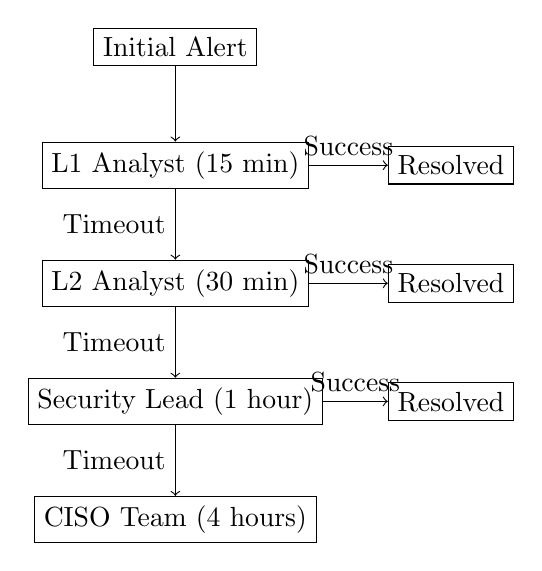
\begin{tikzpicture}[node distance=1.5cm]
      \node (start) [draw, rectangle] {Initial Alert};
      \node (l1) [draw, rectangle, below of=start] {L1 Analyst (15 min)};
      \node (resolved1) [draw, rectangle, right of=l1, xshift=2cm] {Resolved};
      \node (l2) [draw, rectangle, below of=l1] {L2 Analyst (30 min)};
      \node (resolved2) [draw, rectangle, right of=l2, xshift=2cm] {Resolved};
      \node (l3) [draw, rectangle, below of=l2] {Security Lead (1 hour)};
      \node (resolved3) [draw, rectangle, right of=l3, xshift=2cm] {Resolved};
      \node (ciso) [draw, rectangle, below of=l3] {CISO Team (4 hours)};
      
      \draw[->] (start) -- (l1);
      \draw[->] (l1) -- (resolved1) node[midway, above] {Success};
      \draw[->] (l1) -- (l2) node[midway, left] {Timeout};
      \draw[->] (l2) -- (resolved2) node[midway, above] {Success};
      \draw[->] (l2) -- (l3) node[midway, left] {Timeout};
      \draw[->] (l3) -- (resolved3) node[midway, above] {Success};
      \draw[->] (l3) -- (ciso) node[midway, left] {Timeout};
    \end{tikzpicture}
    \caption{Automated escalation workflow}
  \end{figure}
\end{frame}

% Slide 15
\begin{frame}[fragile]
  \frametitle{Access Management: Enabling/Disabling Services Automatically}
  
  \begin{itemize}
    \item \textbf{Dynamic access management} adjusts permissions and service availability based on contextual factors.
    \item Automated service disabling helps contain security incidents by limiting an attacker's lateral movement.
    \item Risk-based access controls automatically adjust permissions based on threat levels and user behavior.
    \item Temporary access automation provides just-in-time privileges that expire automatically after a specified period.
  \end{itemize}
  
  \begin{block}{Automated access adjustment script}
    \tiny
    \begin{semiverbatim}
# Example: Automatically disable access after suspicious activity
def evaluate_user_risk(user_id):
    risk_score = calculate_risk_score(user_id)
    
    if risk_score > HIGH_RISK_THRESHOLD:
        # Automatically disable high-risk access
        disable_admin_access(user_id)
        require_mfa_reauthentication(user_id)
        create_security_review_ticket(user_id, risk_score)
        notify_security_team(user_id, risk_score)
    \end{semiverbatim}
  \end{block}
\end{frame}

% Slide 16
\begin{frame}
  \frametitle{CI/CD Security: Continuous Integration and Testing}
  
  \begin{itemize}
    \item \textbf{CI/CD (Continuous Integration/Continuous Deployment)} pipelines automate software delivery processes.
    \item Security automation in CI/CD ensures that security testing occurs automatically with every code change.
    \item Automated security gates prevent vulnerable code from reaching production environments.
    \item Scanning automation identifies issues like hardcoded credentials, vulnerable dependencies, and insecure configurations.
  \end{itemize}
  
  \begin{block}{Secure CI/CD Pipeline Components}
    \scriptsize
    \begin{enumerate}
      \item \textbf{Pre-commit checks}: Local security linting before code submission
      \item \textbf{Static Application Security Testing (SAST)}: Analyzes source code for vulnerabilities
      \item \textbf{Software Composition Analysis (SCA)}: Checks dependencies for known vulnerabilities
      \item \textbf{Dynamic Application Security Testing (DAST)}: Tests running applications for vulnerabilities
      \item \textbf{Infrastructure as Code scanning}: Validates secure configuration
    \end{enumerate}
  \end{block}
\end{frame}


% Slide 17
\begin{frame}[fragile]
  \frametitle{APIs: Building Blocks of Security Automation}
  
  \begin{itemize}
    \item \textbf{Application Programming Interfaces (APIs)} allow different security tools to communicate and work together.
    \item Security automation depends on robust APIs to integrate diverse security tools into cohesive workflows.
    \item API-driven security enables organizations to build customized security processes across multiple platforms.
    \item Modern security tools should be evaluated partly on the quality and completeness of their API capabilities.
  \end{itemize}
  
  \begin{block}{API example for security integration}
    \tiny
    \begin{semiverbatim}
# Example: Using an API to check if an IP is malicious
curl -X GET "https://api.securityservice.com/v1/reputation/ip/93.184.216.34" \\
  -H "Authorization: Bearer $API_KEY" \\
  -H "Content-Type: application/json"

# Response will contain threat intelligence that can
# be automatically processed and acted upon
    \end{semiverbatim}
  \end{block}
\end{frame}

% Slide 18
\begin{frame}
  \frametitle{Time as a Resource: Efficiency Gains Through Automation}
  
  \begin{itemize}
    \item Security teams typically spend 50-75\% of their time on repetitive tasks that could be automated.
    \item \textbf{Time-to-value} in security operations is dramatically reduced when routine processes are automated.
    \item Analyst time is a finite and expensive resource that should be focused on high-value security activities.
    \item Organizations with mature security automation report handling 3-5 times more security events with the same staff.
  \end{itemize}
  
  \begin{table}
    \scriptsize
    \centering
    \begin{tabular}{|l|r|r|r|}
      \hline
      \textbf{Task} & \textbf{Manual Time} & \textbf{Automated Time} & \textbf{Savings} \\
      \hline
      User onboarding & 45 min & 2 min & 96\% \\
      Alert triage & 15 min & 30 sec & 97\% \\
      Vulnerability verification & 20 min & 1 min & 95\% \\
      Access review & 30 min & 3 min & 90\% \\
      Security reporting & 4 hours & 5 min & 98\% \\
      \hline
    \end{tabular}
    \caption{Time savings through security automation}
  \end{table}
\end{frame}

% Slide 19
\begin{frame}
  \frametitle{Baseline Security: Enforcing Minimum Standards}
  
  \begin{itemize}
    \item \textbf{Security baselines} define the minimum security requirements that must be consistently applied.
    \item Automated enforcement ensures that all systems comply with organizational security standards at all times.
    \item Continuous validation automatically identifies and flags systems that drift from the required baseline.
    \item Remediation automation can automatically correct systems that fall below the defined security baseline.
  \end{itemize}
  
  \begin{exampleblock}{Example: Automated Baseline Controls}
    \scriptsize
    An organization's automated baseline might ensure:
    \begin{itemize}
      \item All systems have endpoint protection installed and updated
      \item All cloud storage is encrypted and not publicly accessible
      \item All accounts require MFA for administrative access
      \item All systems run authorized operating system versions
      \item All web applications implement standard security headers
    \end{itemize}
  \end{exampleblock}
\end{frame}

% Slide 20
\begin{frame}
  \frametitle{Infrastructure Consistency: Templates and Configuration Management}
  
  \begin{itemize}
    \item \textbf{Configuration management} ensures systems are set up and maintained according to secure standards.
    \item Template-based deployment using automation guarantees that all new systems start in a secure state.
    \item Automated configuration validation continuously verifies that security settings remain as intended.
    \item Drift detection identifies when configurations have changed from their approved secure state.
  \end{itemize}
  
  \begin{block}{Configuration Management Process}
    \scriptsize
    \begin{enumerate}
      \item \textbf{Define}: Create secure configuration templates
      \item \textbf{Deploy}: Automatically apply templates to systems
      \item \textbf{Monitor}: Continuously check for configuration compliance
      \item \textbf{Remediate}: Automatically correct deviations
      \item \textbf{Report}: Document compliance status for auditing
    \end{enumerate}
  \end{block}
\end{frame}

% Slide 21
\begin{frame}
  \frametitle{Secure Scaling: Growing Without Increasing Risk}
  
  \begin{itemize}
    \item Business growth typically means more systems, users, and data—all of which expand the attack surface.
    \item \textbf{Secure scaling} means growing the organization while maintaining or improving security posture.
    \item Manual security processes break down as organizations grow, creating security gaps.
    \item Automated security controls scale proportionally with the organization's IT infrastructure.
  \end{itemize}
  
  \begin{figure}
    \centering
    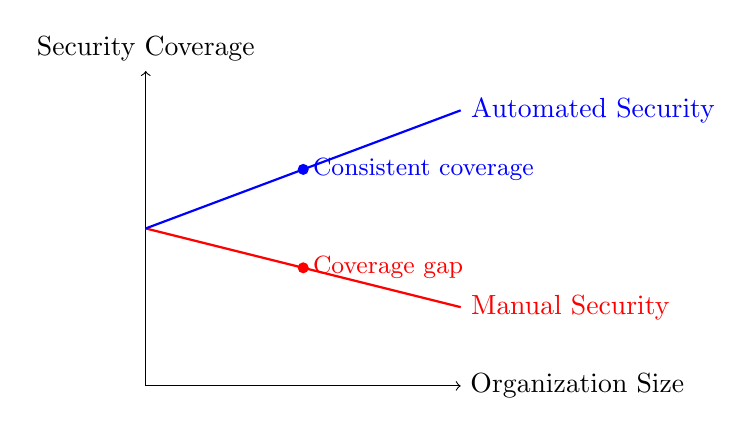
\begin{tikzpicture}
      % Manual scaling line (red)
      \draw[->] (0,0) -- (4,0) node[right] {Organization Size};
      \draw[->] (0,0) -- (0,4) node[above] {Security Coverage};
      \draw[red, thick] (0,2) -- (4,1) node[right] {Manual Security};
      \draw[blue, thick] (0,2) -- (4,3.5) node[right] {Automated Security};
      
      % Add key points
      \fill[red] (2,1.5) circle (2pt) node[right] {\small Coverage gap};
      \fill[blue] (2,2.75) circle (2pt) node[right] {\small Consistent coverage};
    \end{tikzpicture}
    \caption{Security coverage as organizations scale}
  \end{figure}
\end{frame}

% Slide 22
\begin{frame}
  \frametitle{From Repetition to Innovation: Employee Retention}
  
  \begin{itemize}
    \item Security professionals often leave positions due to burnout from repetitive, low-value tasks.
    \item \textbf{Security analyst burnout} is characterized by high turnover rates (often 30\%+ annually) in security operations.
    \item Automation removes tedious work, allowing security staff to focus on challenging and rewarding activities.
    \item Organizations with mature security automation report significantly higher retention rates for security staff.
  \end{itemize}
  
  \begin{alertblock}{Security Team Activities}
    \scriptsize
    \begin{tabular}{|p{0.45\textwidth}|p{0.45\textwidth}|}
      \hline
      \textbf{Low-Value Tasks to Automate} & \textbf{High-Value Tasks for Humans} \\
      \hline
      Alert triage and false positive filtering & Threat hunting and investigation \\
      Report generation and distribution & Strategic security planning \\
      Policy compliance checking & Security architecture design \\
      Log correlation and basic analysis & Advanced attack pattern analysis \\
      Routine vulnerability scanning & Red team/penetration testing \\
      \hline
    \end{tabular}
  \end{alertblock}
\end{frame}

% Slide 23
\begin{frame}
  \frametitle{Faster Response: Automating Incident Handling}
  
  \begin{itemize}
    \item \textbf{Incident response time} directly impacts the damage caused by security breaches.
    \item Each hour of response delay increases the financial impact of a security incident by approximately 2.1\%.
    \item Automated incident response can execute predefined playbooks 24/7 without human delay.
    \item Initial containment actions can be automated to limit damage while human analysts investigate further.
  \end{itemize}
  
  \begin{block}{Automated Incident Response Steps}
    \scriptsize
    \begin{enumerate}
      \item \textbf{Detection}: Automated correlation identifies potential incidents
      \item \textbf{Analysis}: Automated enrichment gathers context about the incident
      \item \textbf{Containment}: Automatic isolation of affected systems
      \item \textbf{Eradication}: Preset response actions remove threats
      \item \textbf{Recovery}: Orchestrated restoration of systems
      \item \textbf{Learning}: Automated documentation for future improvement
    \end{enumerate}
  \end{block}
\end{frame}

% Slide 24
\begin{frame}
  \frametitle{Workforce Multiplication: Doing More With Less}
  
  \begin{itemize}
    \item The global cybersecurity workforce gap exceeds 3.5 million positions, making it impossible to hire enough staff.
    \item \textbf{Workforce multiplication} uses automation to enable each security professional to accomplish more.
    \item Tier-1 security analysts can handle 5-10 times more alerts when supported by proper automation.
    \item Security orchestration allows a small team to implement enterprise-grade security operations.
  \end{itemize}
  
  \begin{exampleblock}{Example: SOC Scaling with Automation}
    \scriptsize
    A 5-person SOC team with mature automation can achieve similar coverage to a 15-20 person team using manual processes by:
    \begin{itemize}
      \item Automating 80\% of routine alert handling
      \item Using playbooks for standard investigations
      \item Implementing automated data enrichment
      \item Deploying self-healing security controls
      \item Automating regular compliance reporting
    \end{itemize}
  \end{exampleblock}
\end{frame}

% Slide 25
\begin{frame}
  \frametitle{Beyond the Basics: Managing Automation Complexity}
  
  \begin{itemize}
    \item \textbf{Automation complexity} increases as more security processes and integrations are added.
    \item Complex automation systems can become difficult to understand, maintain, and troubleshoot.
    \item Security automation should be built incrementally, starting with simple, high-value processes.
    \item Documentation and change management become critical as automation complexity increases.
  \end{itemize}
  
  \begin{block}{Automation Complexity Management}
    \begin{tabular}{|l|l|}
      \hline
      \textbf{Challenge} & \textbf{Mitigation Strategy} \\
      \hline
      Difficult to understand & Modular design with clear documentation \\
      Hard to troubleshoot & Comprehensive logging and monitoring \\
      Challenging to modify & Version control and change management \\
      Knowledge silos & Cross-training and pair programming \\
      \hline
    \end{tabular}
  \end{block}
\end{frame}

% Slide 26
\begin{frame}
  \frametitle{ROI of Automation: Understanding the Cost Equation}
  
  \begin{itemize}
    \item Security automation requires investment in platforms, development time, and ongoing maintenance.
    \item \textbf{Return on investment (ROI)} for security automation involves both tangible and intangible benefits.
    \item Initial automation costs can be significant, but are typically recouped within 12-18 months.
    \item Organizations should prioritize automation projects based on potential security impact and cost savings.
  \end{itemize}
  
  \begin{exampleblock}{Security Automation ROI Calculation}
    \scriptsize
    \begin{align*}
      \text{ROI} &= \frac{\text{Value of Benefits} - \text{Total Costs}}{\text{Total Costs}} \times 100\% \\
      \text{Where:} \\
      \text{Benefits} &= \text{Time Saved} + \text{Incident Cost Reduction} + \text{Reduced Risk} \\
      \text{Costs} &= \text{Software} + \text{Implementation} + \text{Maintenance} + \text{Training}
    \end{align*}
  \end{exampleblock}
\end{frame}

% Slide 27
\begin{frame}[fragile]
  \frametitle{Single Points of Failure: Avoiding Automation Pitfalls}
  
  \begin{itemize}
    \item Automated security systems can become \textbf{single points of failure (SPOF)} if not designed with redundancy.
    \item Dependency on a single automation platform creates risk if that platform experiences downtime or vulnerabilities.
    \item Security automation should include monitoring of the automation system itself to detect failures.
    \item Manual fallback procedures must be documented for critical security functions if automation fails.
  \end{itemize}
  
  \begin{block}{Automation Failure Example}
    \tiny
    \begin{semiverbatim}
# Example: Monitoring the automation system
def check_automation_health():
    for component in automation_components:
        status = component.get_status()
        if status != "operational":
            # Execute recovery procedure
            recovery_procedure(component)
            
            # Notify security team
            alert_security_team(f"Automation failure in {component.name}")
            
            # Activate manual fallback if needed
            if component.criticality == "high":
                activate_manual_fallback(component)
    \end{semiverbatim}
  \end{block}
\end{frame}

% Slide 28
\begin{frame}
  \frametitle{Technical Debt: Balancing Quick Wins vs. Long-term Solutions}
  
  \begin{itemize}
    \item \textbf{Technical debt} in security automation occurs when shortcuts are taken to deploy automation quickly.
    \item Scripts and automations created as "temporary solutions" often become permanent but unmaintainable.
    \item Legacy automation systems can become security risks themselves if not properly maintained and updated.
    \item Sustainable security automation requires investment in proper architecture, testing, and documentation.
  \end{itemize}
  
  \begin{alertblock}{Signs of Security Automation Technical Debt}
    \scriptsize
    \begin{itemize}
      \item Undocumented scripts running critical security functions
      \item Automation that only one person understands
      \item Fragile integrations that break when systems update
      \item Hard-coded credentials or outdated authentication methods
      \item Lack of testing environments for automation changes
      \item Inconsistent error handling and logging
    \end{itemize}
  \end{alertblock}
\end{frame}

% Slide 29
\begin{frame}
  \frametitle{Supportability: Maintaining Your Automation Infrastructure}
  
  \begin{itemize}
    \item \textbf{Supportability} refers to how easily security automation can be maintained over time.
    \item Automation maintenance requires ongoing investment as security tools, threats, and business needs evolve.
    \item Long-term automation success depends on proper documentation, monitoring, and knowledge transfer.
    \item Organizations often underestimate the resources needed to maintain security automation systems.
  \end{itemize}
  
  \begin{block}{Automation Supportability Best Practices}
    \scriptsize
    \begin{enumerate}
      \item Create thorough documentation for all automation processes
      \item Implement comprehensive logging and monitoring
      \item Develop testing procedures for automation updates
      \item Establish clear ownership and responsibility
      \item Plan for periodic review and refactoring
      \item Ensure multiple team members understand each automation
    \end{enumerate}
  \end{block}
\end{frame}

% Slide 30
\begin{frame}
  \frametitle{Building Your Automation Roadmap}
  
  \begin{itemize}
    \item A successful security automation journey requires strategic planning rather than ad-hoc implementation.
    \item \textbf{Automation roadmaps} outline the sequence and dependencies of automation initiatives over time.
    \item Start with high-value, lower-complexity automations to build momentum and demonstrate value.
    \item Plans should include capability building (tools, skills, processes) alongside specific automations.
  \end{itemize}
  
  \begin{table}
    \scriptsize
    \begin{tabular}{|l|l|l|}
      \hline
      \textbf{Phase} & \textbf{Focus Areas} & \textbf{Timeline} \\
      \hline
      Foundation & Basic user provisioning, vulnerability scanning & 0-3 months \\
      \hline
      Core Security & Alert triage, incident response, access control & 3-9 months \\
      \hline
      Advanced & CI/CD integration, threat hunting, SOAR & 9-18 months \\
      \hline
      Optimization & Machine learning, advanced analytics, tuning & 18+ months \\
      \hline
    \end{tabular}
    \caption{Example Security Automation Roadmap Phases}
  \end{table}
\end{frame}

% Slide 31
\begin{frame}
  \frametitle{Starting Small: First Steps in Security Automation}
  
  \begin{itemize}
    \item Begin by identifying repetitive, time-consuming security tasks that are good automation candidates.
    \item \textbf{Process mapping} documents existing security workflows before automating them.
    \item The "crawl-walk-run" approach builds automation maturity incrementally, with manageable milestones.
    \item Early wins help build organizational support for more advanced automation initiatives.
  \end{itemize}
  
  \begin{exampleblock}{Starter Automation Projects}
    \scriptsize
    These automation projects offer high value with moderate complexity:
    \begin{itemize}
      \item Basic user onboarding/offboarding workflow
      \item Automated vulnerability scan scheduling and reporting
      \item Simple alert enrichment with context from multiple sources
      \item Scheduled security compliance checks and reporting
      \item Automated response to common, low-risk security alerts
    \end{itemize}
  \end{exampleblock}
\end{frame}

% Slide 32
\begin{frame}
  \frametitle{Future Trends: Where Security Automation Is Heading}
  
  \begin{itemize}
    \item \textbf{Machine learning} is increasingly incorporated into security automation for anomaly detection and decision support.
    \item Self-healing security systems can automatically remediate issues without human intervention.
    \item Automation is extending beyond prevention and detection to include autonomous response capabilities.
    \item The future security operations center will feature humans supervising automated systems rather than performing tasks directly.
  \end{itemize}
  
  \begin{alertblock}{Key Takeaways}
    \scriptsize
    \begin{itemize}
      \item Security automation is no longer optional—it's essential for effective security operations
      \item Start with clear security goals, not technology for its own sake
      \item Build incrementally from simple to complex automations
      \item Consider the full lifecycle including maintenance and updates
      \item Focus automation on freeing humans for high-value security work
    \end{itemize}
  \end{alertblock}
\end{frame}

\end{document}